\documentclass[../../main.tex]{subfiles}
\begin{document}
\onlyinsubfile{
\setcounter{chapter}{1}
}
\notinsubfile{}
%
\chapter{Waar is het qubit?}\label{chap:H2}
\marginpar{
\includegraphics[width=0.4\textwidth]{./img/sherlockwatson.jpg}\par
}
In dit hoofdstuk gaan we op zoek naar het qubit. We onderzoeken eerst hoe een klassieke computer met bits werkt. We leren rekenen met een twee-toestandsysteem en hoe je er mee kunt rekenen op de eenheidscirkel. We leren te wisselen van basis. Deze stap hebben we nodig om het verschil tussen klassieke bits en quantum bits uit te leggen. Het hoofdstuk sluit af met een lijst met criteria waar een quantumcomputer aan moet voldoen. 

\section{Van bits ...}\label{sec:vanbit}

\begin{flushleft}
\begin{minipage}{.45\textwidth}
\includegraphics[width=\textwidth]{./img/alu.png}
\end{minipage}%
\hfill
\begin{minipage}{.5\textwidth}
\captionof{figure}{Een zeer vereenvoudigde centrale verwerkingseenheid (central processing unit, CPU). Het hart van een klassieke computer.\label{fig:alu}}
\end{minipage}
\end{flushleft}

Een klassieke computer verwerkt reeksen nullen en enen, die soms gegevens en soms instructies voorstellen. Een processor transformeert de reeks naar een andere reeks. Daarbij worden ook nullen en enen naar het geheugen geschreven en opgehaald uit het geheugen. Tot op de dag van vandaag werken bijna alle computers volgens dit systeem dat in 1945 is uitgedacht door John von Neumann~\cite{Neumann1945}. In dit \hrefqr[-2cm]{https://www.futurelearn.com/courses/how-computers-work/0/steps/49284}{filmpje} van 4 minuten wordt een berekening uitgevoerd die op jouw computer makkelijk binnen enkele nanoseconden wordt uitgevoerd. 

Klassieke computers beschikken over de volgende kenmerken:
\begin{itemize}
\item Ze werken met bits. Een bit is de elementaire informatiedrager die nul of \'e\'en kan zijn. Het antwoord op een vraag die met ja of nee kan worden beantwoord bevat \'e\'en bit informatie. E\'en Megabit bevat dus de informatie van een miljoen ja/nee-vragen.  
\item Ze maken gebruik van een verwerker. Deze beschikt over logische poorten die een reeks nullen en enen kunnen veranderen in een andere reeks nullen en enen.
\item Er is een set poorten waarmee je elke logische schakeling kunt maken. Een universele set is bijvoorbeeld te maken met de EN en de NOT poort en de mogelijkheid om de uitkomst van \'e\'en poort naar twee of meer andere poorten door te sturen als input. 
\item Met de vorige eigenschap kunnen bits dus gekopieerd worden. 
\item Je kunt bits in een permanent geheugen bewaren. 
\end{itemize}

 In werkblad~\ref{sec:wbklassiek} leer je werken met klassieke poorten. De verwerker beschikt over logische poorten. Als je hier iets meer over wilt weten dan moet je het experiment bij werkblad~\ref{sec:wbklassiek} uitvoeren.

\begin{experiment}{Klassieke bits}
Voer werkblad~\ref{sec:wbklassiek} uit.
\end{experiment}

De quantumcomputer verschilt van de klassieke computer:
\begin{itemize}

\item Een quantumcomputer werkt niet met bits maar met qubits. In dit hoofdstuk gaan we verkennen wat daar de eigenschappen van zijn. 
\item De quantumcomputer kent wel poorten, maar die zien er heel anders uit. In hoofdstuk~\ref{chap:H3} zullen we die verkennen. 
\item Kopi\"eren van een qubit is niet mogelijk, dus een quantumpoort kan maar aan \'e\'en poort informatie doorgeven.
\end{itemize}

Kortom, klassieke computers kunnen dingen die quantumcomputers niet kunnen. Quantumcomputers zullen klassieke computers niet vervangen. Maar die quantumcomputers kunnen dingen die klassieke computers niet kunnen\ldots

\section{... naar qubits}\label{sec:qubit}
Quantumcomputers hebben hun eigen elementaire informatiedrager, het quantumbit ofwel qubit. Ook het qubit kent twee basistoestanden. In werkblad~\ref{sec:wbYoung2} maakten we al kennis met de superpositie van fotonen die in het dubbelspleetexperiment zowel horizontaal als verticaal gepolariseerd waren. Om een idee te krijgen wat dit betekent kijken we naar een model voor superpositie uit de klassieke wereld. Bekijk figuur~\ref{fig:ovjv}. 

\begin{center}
\leavevmode
\includegraphics[width=0.5\textwidth]{./img/ovjv.png}
 \captionof{figure}{Wat is hier afgebeeld?)
\label {fig:ovjv}}
\end{center}

De afbeelding heette in 1915 ``My Wife and My Mother-in-Law''~\cite{Hill1915} naar een Duitse ansichtkaart uit 1888. De tekening zou men kunnen beschouwen als een superpositie van de afbeeldingen van een jonge vrouw en van een oude vrouw. Maar als je gaat kijken, en dus een meting doet,  dan zie je slechts \'e\'en van de twee. 
Onze hersenen kunnen kennelijk maar \'e\'en van de twee beelden tegelijk verwerken. 

\begin{experiment}{Oude vrouw Jonge vrouw}
Voer het eerste deel van werkblad~\ref{sec:wbOVJV} uit.
\end{experiment}

Het plaatje is een objectief gegeven. De tekenaar heeft zijn best gedaan de oude en de jonge vrouw allebei tot uiting te laten komen. We kunnen de inhoud 'oud en jong' in het plaatje als een vector voorstellen in een willekeurige maar vaste richting. In figuur~\ref{fig:ovjvvector} is dat met een rode pijl weergegeven.

Waarnemers scoren verschillende percentages oude of jonge vrouw. Hoe waarnemers het plaatje interpreteren is het resultaat van de test: het percentage 'oud' en 'jong'.

\begin{center}
\leavevmode
\begin{figure}[h]
\def\ojfrangle{10}
\def\ojobangle{70}
\def\ojscale{.33}
\begin{tikzpicture}%
\begin{scope}[scale=\ojscale, rotate=\ojfrangle]
  \draw[thin,gray!40] (-0.1,-0.1) grid (5,5);
  \draw[-stealth] (-0.1,0)--(5,0) node[midway, below, xshift=10]{${\scriptstyle\ket{O_1}}$};
  \draw[-stealth] (0,-0.1)-- (0,5) node[midway, left, yshift=-10]{${\scriptstyle\ket{J_1}}$};
  \draw[line width=.1pt ,black] ([shift=(0:5)]0,0) arc (0:90:5);
  \draw[thick, blue, -stealth](0,0)--($cos(\ojobangle-\ojfrangle)*(5,0)$) node(x){};
  \draw[thick, blue, -stealth](0,0)--($sin(\ojobangle-\ojfrangle)*(0,5)$) node(y){};
  \draw[thick, red, -stealth](0,0)--(\ojobangle-\ojfrangle:5) node (p){};
  \draw[loosely dashed] (x)--(p);
  \draw[loosely dashed] (y)--(p);
\end{scope}
  \node [below] at (0,0) {$1$};
\end{tikzpicture}
\def\ojfrangle{50}
\begin{tikzpicture}
\begin{scope}[scale=\ojscale,  rotate=\ojfrangle]
  \draw[thin,gray!40] (-0.1,-0.1) grid (5,5);
  \draw[-stealth] (-0.1,0)--(5,0) node[midway, below, xshift=10]{${\scriptstyle\ket{O_2}}$};
  \draw[-stealth] (0,-0.1)-- (0,5) node[midway, left, yshift=-10]{${\scriptstyle\ket{J_2}}$};
  \draw[line width=.1pt ,black] ([shift=(0:5)]0,0) arc (0:90:5);
  \draw[thick, blue, -stealth](0,0)--($cos(\ojobangle-\ojfrangle)*(5,0)$) node(x){};
  \draw[thick, blue, -stealth](0,0)--($sin(\ojobangle-\ojfrangle)*(0,5)$) node(y){};
  \draw[thick, red, -stealth](0,0)--(\ojobangle-\ojfrangle:5) node (p){};
  \draw[loosely dashed] (x)--(p);
  \draw[loosely dashed] (y)--(p);
\end{scope}
  \node [below] at (0,0) {$2$};
\end{tikzpicture}
\def\ojfrangle{-20}
\begin{tikzpicture}
\begin{scope}[scale=\ojscale,  rotate=\ojfrangle]
  \draw[thin,gray!40] (-0.1,-0.1) grid (5,5);
  \draw[-stealth] (-0.1,0)--(5,0) node[midway, below, xshift=4, scale=.7]{$\ket{O_3}$};%aangepast
  \draw[-stealth] (0,-0.1)-- (0,5) node[midway, left, yshift=-10]{${\scriptstyle\ket{J_3}}$};
  \draw[line width=.1pt ,black] ([shift=(0:5)]0,0) arc (0:90:5);
%  \draw[thick, blue, -stealth](0,0)--($cos(\ojobangle-\ojfrangle)*(5,0)$) node(x){};
  \draw[thick, blue, -stealth](0,0)--($sin(\ojobangle-\ojfrangle)*(0,5)$) node(y){};
  \draw[thick, red, -stealth](0,0)--(\ojobangle-\ojfrangle:5) node (p){};
%  \draw[loosely dashed] (x)--(p);
%  \draw[loosely dashed] (y)--(p);
\end{scope}
  \node [below, xshift=.3cm, yshift=-.4cm] at (0,0) {$3$};
\end{tikzpicture}
\def\ojfrangle{70}
\begin{tikzpicture}
 \begin{scope}[scale=\ojscale,rotate=\ojfrangle]
  \draw[thin,gray!40] (-0.1,-0.1) grid (5,5);
  \draw[-stealth] (-0.1,0)--(5,0) node[midway, below, xshift=10]{${\scriptstyle\ket{O_4}}$};
  \draw[-stealth] (0,-0.1)-- (0,5) node[midway, left, yshift=-10]{${\scriptstyle\ket{J_4}}$};
  \draw[line width=.1pt ,black] ([shift=(0:5)]0,0) arc (0:90:5);
  \draw[thick, blue, -stealth](0,0)--($cos(\ojobangle-\ojfrangle)*(5,0)$) node(x){};
%  \draw[thick, blue, -stealth](0,0)--($sin(\ojobangle-\ojfrangle)*(0,5)$) node(y){};
  \draw[thick, red, -stealth](0,0)--(\ojobangle-\ojfrangle:5) node (p){};
%  \draw[loosely dashed] (x)--(p);
%  \draw[loosely dashed] (y)--(p);
 \end{scope}
  \node [below] at (0,0) {$4$};
\end{tikzpicture}
\caption{Resultaten van vier waarnemers van ``oude vrouw/jonge vrouw''. het object (rode pijl) is voor alle waarnemers gelijk. Bij elke waarnemer hoort een eigen assenstelsel.}
\label{fig:ovjvvector}
\end{figure}
\end{center}
In figuur~\ref{fig:ovjvvector} hebben vier waarnemers ($W$) een tijdje naar hetzelfde plaatje gekeken. $W_1$ ziet vaker een jonge vrouw en $W_2$ heeft een grote kans om een oude vrouw te zien. $W_3$ ziet met zekerheid een jonge vrouw. En $W_4$ ziet met zekerheid een oude vrouw.
 
Het nut van deze abstracte voorstelling is dat deze gebruik maakt van dezelfde wiskundige taal als de quantumtheorie. Het assenstelsel is dan karakteristiek voor de waarnemer.

\marginpar{\vspace{0cm}\footnotesize{De notatie $\ket{0}$ en $\ket{1}$ lijkt op de pijl van een vector. Dit is de \textit{braket} notatie van Paul Dirac, een Brits natuurkundige en een pionier in de quantumtheorie.}}

De twee toestanden 'oud' en 'jong' zouden we als klassieke bits kunnen opvatten. Hier gebruikt de waarnemer een vectorruimte om verschillende toestanden ten opzichte van elkaar vast te leggen. Die vectorruimte wordt opgespannen met twee basisvectoren die elkaar uitsluiten. Voor de eerste waarnemer zijn dat $\ket{J_1}$ en $\ket{O_1}$. Op basis van figuur~\ref{fig:ovjvvector} geldt blijkbaar (meet de relatieve amplitudes maar na):

\marginpar{\vspace{0cm}\footnotesize{De co\"effici\"enten noem je \textit{amplitudes}, hun kwadraten geven de \textit{kans}.}}

\[\ket{\Psi_{JO}} = \num{0,87}\ket{J_1} +  \num{0,5}\ket{O_1}\]
De Griekse letter $\Psi$ (spreek uit: psi) wordt in de quantumwereld vaak gebruikt om een toestand uit te drukken. Herken je de vectoroptelling die je ook gebruikt als je bijvoorbeeld krachten optelt? De co\"effici\"enten geven de lengtes aan van de projecties op de assen. De toestandsvectoren hebben altijd een lengte 1. De stelling van Pythagoras leert: 
\[\num{0,87}^2 + \num{0,5}^2 = \num{0,75} + \num{0,25}  = \num{1}\]  
Bedenk dat de waarnemer \`ofwel een jonge vrouw \`ofwel een oude vrouw ziet. Er geldt dus dat (kans op een oude vrouw) + (kans op een jonge vrouw) = \SI{100}{\percent}. 
In dit voorbeeld geldt blijkbaar dat waarnemer~1 een kans van \SI{75}{\percent} heeft om een jonge vrouw te zien en een kans van \SI{25}{\percent} om een oude vrouw te zien. 

Pas op! De afbeelding van figuur~\ref{fig:ovjv} is geen qubit. Het is geen quantumobject. 
\medskip
\begin{opdracht}\label{opd:inzoomen}%
Hoeveel machten van tien zouden we moeten inzoomen om van het plaatje tot in de quantumwereld te komen?
\end{opdracht}
\begin{antwoord}[-3cm]
Je moet afdalen tot de \textit{nanowereld}. Dat is de wereld van molekulen en atomen. Een atoom is ongeveer \SI{0.1}{\nano\meter} groot. Minstens een factor $\num{1E9}$ dus.
\end{antwoord}

Het model lijkt een superpositie van twee toestanden te dragen. Bij een waarneming zie je maar \'e\'en van de twee. We kunnen de kans en amplitude beschrijven en weergeven in een vectorvoorstelling zoals in het tweede deel van experiment~\ref{sec:wbOVJV}.
\medskip
\begin{experiment}{Oude vrouw Jonge vrouw}
Voer het tweede deel van werkblad~\ref{sec:wbOVJV} uit.
\end{experiment}
Maar het blijft een metafoor, we hebben nog geen stap in de quantumwereld gezet. Het wordt tijd om te kijken naar een echt qubit.

\section{Hier is het qubit}\label{sec:zoekqubit}

We zetten even op een rijtje wat onze verkenningen tot nu toe hebben opgeleverd.

\begin{itemize}
\item In hoofdstuk~\ref{chap:H1} hebben we \textit{interferentie} gevonden bij het enkel- en dubbelspleetexperiment, een bewijs voor het golfkarakter van licht.

\item We gebruikten Einsteins bevinding dat licht opgebouwd is uit deeltjes (energiepakketjes) die we nu fotonen noemen. In een simulatie zagen we dat het gedrag van individuele fotonen niet voorspelbaar is, maar dat zij wel een kansverdeling volgen. Als je heel veel fotonen projecteert wordt deze kansverdeling in het intensiteitspatroon zichtbaar.

\item We onderzochten polarisatie, een eigenschap die alleen bij transversale golven kan optreden. Als ongepolariseerd licht door een polarisatiefilter gaat, wordt de helft tegengehouden en de helft die doorgelaten wordt krijgt de polarisatierichting van het filter. Alle doorgelaten fotonen hebben nu dezelfde polarisatierichting. De bundel is \textit{geprepareerd}. In figuur~\ref{fig:photonvector} valt een bundel licht die gepolariseerd is in de richting van de pijl op een polarisatiefilter. De doorlaatrichting van het filter is de lange as, die een hoek $\theta$ maakt met de lichtbundel. De kans om doorgelaten te worden is evenredig met $\cos^2 \theta$. We toonden dit aan in werkblad~\ref{sec:wbmalus} door gepolariseerd licht van een computerscherm te gebruiken.
\end{itemize}

\marginpar{\vspace{0cm}\footnotesize{De wet van Malus:\\ $I=I_0 cos^2 \theta$}}

\begin{flushleft}
%\leavevmode
\begin{minipage}{.45\textwidth}
\includegraphics[width=\textwidth]{./img/photonvector.png}
\end{minipage}%
\hfill
\begin{minipage}{.5\textwidth}
\captionof{figure}{De polarisatierichting is in de lengterichting van het blauwe kristal. Een foton in de toestand $\ket{1}$ zal het filter passeren.
Een foton in de toestand $\ket{0}$ wordt tegengehouden. Het foton in de afbeelding heeft een kans van $\cos^2 \theta$ om te worden doorgelaten.\label{fig:photonvector}}
\end{minipage}
%\caption{E\'en vector in standaardbasis (rood) en diagonale basis.}\label{fig:hvad}
%\end{figure}
\end{flushleft}

Aan het tweede filter kunnen we nu een co\"ordinatenstelsel toewijzen (zie figuur~\ref{fig:photonvector}). Toestand $\ket{1}$ wordt zeker doorgelaten, en toestand  $\ket{0}$ wordt zeker geblokkeerd. Aan elke toestand wijzen we nu een vector toe met lengte 1 en een richting die overeenkomt met de polarisatierichting van die toestand. In de vierde klas heb je geleerd dat in figuur~\ref{fig:photonvector} moet gelden:

\[\ket{\Psi}=\sin\theta\ket{0}+\cos\theta\ket{1}\]

In een andere notatie, als we voor $\sin\theta=\alpha$ en $\cos\theta=\beta$ invullen,  en de basisvectoren schrijven als $\ket{0} = \smqty(1\\0)$ en\\ $\ket{1} = \smqty(0\\1)$, schrijven we ook wel: 
\[\begin{aligned}
\ket{\Psi}&=\alpha\ket{0}+\beta\ket{1}\\
\ket{\Psi}&=\mqty(\sin\theta \\ \cos\theta)=\mqty(\alpha \\ \beta)
\end{aligned}\]

We kunnen de toestand van het foton dus opvatten als een superpositie van de basistoestanden. 'Het foton is als het ware in twee toestanden tegelijkertijd'. Dit is een eigenschap die een klassiek bit niet heeft, dat is immers altijd 0 of 1. De kans dat het foton wordt doorgelaten is dan blijkbaar gelijk aan  $\beta^2$. Er is natuurlijk ook een  kans dat het foton door het tweede filter juist wordt tegengehouden. De beide kansen samen moeten optellen tot 1. De kans op tegenhouden moet dan wel gelijk zijn aan het kwadraat van de co\"effici\"ent van de toestand $\ket{0}$.  Er geldt immers 

\[\cos^2\theta + \sin^2\theta=1 , \quad \alpha^2+\beta^2=1\]

Elke toestand kan als een vector op de eenheidscirkel worden geschreven. In figuur~\ref{fig:photonvector} zagen we dat al.

In figuur~\ref{fig:eenheidscirkel} is de eenheidscirkel nogmaals getekend. Elk punt op de eenheidscirkel correspondeert met een toestand. Er zijn oneindig veel toestanden want er zijn oneindig veel punten op een cirkel. Van acht toestanden is de bijbehorende vector getekend. 

\begin{flushleft}
%\leavevmode
\begin{minipage}{.4\textwidth}
\begin{tikzpicture}[scale=.5]
\def\vectsize{.7}
\def\radius{5cm}
\def\labelrad{6.5cm}
\def\ketrad{6.5cm}
\def\arrowrad{3cm}
\draw[thin,gray!40] (-5,-5) grid (5,5);
\draw (0,0) circle (\radius);
\foreach \x in {0,90} \filldraw (\x:\radius) circle (.1);
\foreach \x in {0,1,2,3,4,5,6,7} \draw[thick, red, -stealth](0,0)--( 45*\x:\radius);
%\draw[thick, red, -stealth](0,0)--(45:\radius);
%\draw[thick, red, -stealth](0,0)--(90:\radius);
%\draw[thick, red, -stealth](0,0)--(90:\radius);
%\node[scale=1] at (-5,5.5) {Eenheidscirkel};
%\node[scale=1, label=right:{$\ket{1}$}] at ( 90:\ketrad) {};
%\node[scale=1, label=right:{$\ket{0}$}] at (  0:\ketrad) {};
\node[scale=\vectsize] at ( +90:\labelrad) {$\mqty( 0 \\ 1 )=\ket{1}$};
\node[scale=\vectsize] at ( +45:\labelrad) {$
\mqty( \tfrac{1}{\sqrt{2}} \\ \tfrac{1}{\sqrt{2}} ) =\ket{+}$};
\node[scale=\vectsize] at (   0:\labelrad) {$\mqty( 1 \\ 0 )=\ket{0}$};
\node[scale=\vectsize] at ( -45:\labelrad) {$
\mqty( \tfrac{1}{\sqrt{2}}  \\ \tfrac{-1}{\sqrt{2}} )=\ket{-} $};
\node[scale=\vectsize] at ( -90:\labelrad) {$\mqty( 0 \\ -1 )$};
\node[scale=\vectsize] at (-135:\labelrad) {$
\mqty( \tfrac{-1}{\sqrt{2}}  \\ \tfrac{-1}{\sqrt{2}} ) $};
\node[scale=\vectsize] at ( 180:\labelrad) {$\mqty( -1\\ 0 )$};
\node[scale=\vectsize] at ( 135:\labelrad) {$
\mqty( \tfrac{-1}{\sqrt{2}}  \\ \tfrac{1}{\sqrt{2}} ) $};
\end{tikzpicture}
\end{minipage}%
\hfill
\begin{minipage}{.35\textwidth}
\captionof{figure}{Vectoren die wavuit de oorsprong eindigen op de eenheidscirkel corresponderen met toestanden van een qubit.\label{fig:eenheidscirkel}}
\end{minipage}
\end{flushleft}

Stel nu dat we een foton hebben met een onbekende toestand~${\ket{\Psi}=\smqty(\alpha \\ \beta)}$. Kunnen we door middel van metingen vaststellen wat de toestandsco\"effici\"enten $\alpha$ en $\beta$ zijn?  

De procedure is als volgt. Het filter staat klaar en achter het filter is een fotodetector geplaatst die een klik geeft als er \'e\'en foton opvalt. 
Het foton valt op het filter. Er is nu een kans dat hij er door gaat en dan hoor je een klik. Maar als hij wordt tegengehouden hoor je niets. Dat is alles. Klik of geen klik. Het experiment overdoen kan niet. Het foton is weg, en daarmee de informatie over zijn polarisatietoestand.
 
De enige manier om de toestand van het foton te achterhalen is door het experiment te herhalen met een groot aantal fotonen die allemaal in dezelfde toestand verkeren.  Met behulp van de klikfrequenties kan nu statistiek worden bedreven. Daarover gaat opdracht~\ref{opd:herhaal}. 
\medskip
\begin{opdracht}\label{opd:herhaal}
Een polarisatiefilter staat verticaal opgesteld. Achter het filter staat een fotodetector die een klik geeft als er een foton opvalt. 
Men laat 1000 fotonen op het filter vallen die allemaal op dezelfde wijze zijn geprepareerd. De toestand van de fotonen wordt beschreven met de formule 

\[\begin{aligned}\ket{\Psi}=\alpha\ket{0}+\beta\ket{1}\end{aligned}\]

Er wordt 750 keer een klik vastgesteld. 

\begin{enumerate}
\item  Bereken de co\"effici\"enten $\alpha$ en $\beta$.
\item Bereken de hoek tussen de polarisatierichting van de fotonen en de doorlaatrichting van het filter.
\end{enumerate}
\end{opdracht}
\begin{antwoord}[-8cm]
Het filter meet toestand $\ket{1}$.

$\beta^2=\tfrac{3}{4} \implies$\\ $\beta=\pm\tfrac{1}{2}\sqrt{3}$

$\alpha^2+\beta^2=1 \implies$\\ $\alpha=\pm\tfrac{1}{2}$

toestandsvector: Hoek met verticaal= \SI{30}{\degree} NB er zijn vier mogelijkheden.

\end{antwoord}

\section{Het meten met verschillende bases}\label{sec:verschillendebases}
In het voorgaande zagen we dat de toestand van een qubit kan worden beschreven met behulp van een toestandsvector. Om de toestand te leren kennen zal er gemeten moeten worden. Maar met het meetapparaat komt een meetbasis.  Zo'n meetbasis bestaat uit twee toestanden waarvan de bijbehorende toestandsvectoren loodrecht op elkaar staan. De onderzoeker noemt die twee toestanden doorgaans $\ket{0}$ en $\ket{1}$.  Men spreekt in dat geval van de standaardbasis. Die basis is een vrije keuze. Als er dus twee onderzoekers zijn, die elk hun eigen basis kiezen is het handig om de twee bases te onderscheiden met een subscript, bijvoorbeeld $\ket{0}_A$ en $\ket{1}_A$  voor de \'e\'en en $\ket{0}_B$ en $\ket{1}_B$ voor de ander.

Voor onderzoeker A is de toestand van het qubit gelijk aan 

\[\ket{\Psi} = \alpha \ket{0}_A +\beta\ket{1}_A\]
Voor onderzoeker B is de toestand van het qubit  gelijk aan 
\[\ket{\Psi} = \gamma \ket{0}_B +\delta\ket{1}_B\]

Het verwisselen van bases is een belangrijk instrument in quantumalgoritmes. Naast de standaardbasis wordt vaak de diagonale basis gebruikt die in figuur~\ref{fig:BB84base} is afgebeeld. Voor de diagonale basis gebruiken we meestal $\ket{+}$ en $\ket{+}$:

\[\ket{+} = \ket{1}_B = \ket{1}_{45\si{\degree}}\]
\[\ket{-} = \ket{0}_B = \ket{0}_{45\si{\degree}}\]


\begin{flushleft}
\begin{minipage}{.75\textwidth}
\def\gcolor{green!60!black}
\def\ojfrangle{0}
\def\ojobangle{45}
\def\statangle{30}
\def\ojscale{.65}
\begin{tikzpicture}%
\clip (-1.7,-4) rectangle (4,4);
\begin{scope}[scale=\ojscale, rotate=\ojfrangle]
  \draw[thin,red!40] (-5,-5) grid (5,5);
  \draw[line width=.1pt ,black!30] ([shift=(-90:5)]0,0) arc (-90:180:5);

  \draw[-stealth, gray!40] (0,0) circle (5cm);
  \draw[-stealth, red!40] (-0.1,0)-- (5,0) node[below, red, xshift=10]{${\scriptstyle\ket{0}_A}$};
  \draw[-stealth, red!40] (0,-0.1)-- (0,5) node[left, red, yshift=0]{${\scriptstyle\ket{1}}_A$};
%  \draw[line width=.1pt ,black] ([shift=(0:5)]0,0) arc (0:90:5);
  \draw[thick, red, -stealth](0,0)--($cos(\ojobangle-\statangle)*(5,0)$) node(x)[label={[xshift=-7, yshift=-20]$\alpha$}]{};
  \draw[thick, red, -stealth](0,0)--($sin(\ojobangle-\statangle)*(0,5)$) node(y)[label={[xshift=-10, yshift=-20]$\beta$}]{};
  \draw[thick, blue, -stealth](0,0)--(\ojobangle-\statangle:5) node (p){};
  \draw[red, dashed] (x.center)--(p.center) ;
  \draw[red, dashed] (y.center)--(p.center);
\end{scope}
\def\ojfrangle{-45}
\begin{scope}[scale=\ojscale,  rotate=\ojfrangle]
  \draw[thin,green!40!lightgray] (-5,-5) grid (5,5);
  \draw[-stealth, green!40!gray] (-0.1,0)--(5,0) node[right,  xshift=-3, yshift=-3]{${\scriptstyle\ket{0}_B}$};
  \draw[-stealth,\gcolor] (0,-0.1)-- (0,5) node[above left,  xshift=13]{${\scriptstyle\ket{1}_B}$};
%  \draw[line width=.1pt ,black] ([shift=(0:5)]0,0) arc (0:90:5);
  \node at (\ojobangle-\ojfrangle-\statangle:5)   (p) {}; 
  \draw[thick, \gcolor, -stealth](0,0)--($cos(\ojobangle-\ojfrangle-\statangle)*(5,0)$) node(x)[label={[xshift=-10, yshift=-20]$\delta$}]{};
  \draw[thick, \gcolor, -stealth](0,0)--($sin(\ojobangle-\ojfrangle-\statangle)*(0,5)$) node(y)[label={[xshift=-10, yshift=-10]$\gamma$}]{};
%  \draw[thick, blue!50, -stealth](0,0)--(\ojobangle-\ojfrangle-\statangle:5) node (p){P};
%no need to draw again node suffices
  \draw[\gcolor, dashed] (x)--(p);
  \draw[\gcolor, dashed] (y)--(p);
\end{scope}
\end{tikzpicture}
\end{minipage}%
\hfill
\hspace{{-.25\textwidth}}%
\begin{minipage}{.50\textwidth}
\captionof{figure}{De blauwe toestandsvector wordt in de standaardbasis (rood) genoteerd als $\ket{\Psi} = \alpha \ket{0}_A +\beta\ket{1}_A$
en in de diagonale basis (groen) als $\ket{\Psi} = \gamma \ket{0}_B +\delta\ket{1}_B$
}\label{fig:BB84base}
\end{minipage}
%\caption{E\'en vector in standaardbasis (rood) en diagonale basis.}\label{fig:hvad}
%\end{figure}
\end{flushleft}


\begin{opdracht}\label{opd:basiscoef}
Een onderzoeker beschikt over een qubit in de toestand $\ket{\Psi} = \tfrac{1}{2} \ket{0} +\tfrac{1}{2}\sqrt{3}\ket{1}$. Hij gaat over van de standaardbasis $\ket{0}$ en $\ket{1}$ naar de diagonale basis  $\ket{+}$ en $\ket{-}$. De toestand wordt dan beschreven door $\ket{\Psi} = \gamma\ket{+} +\delta\ket{-}$

\begin{enumerate}
\item Bereken de coëfficiënten $\gamma$ en $\delta$
\item Bereken de kans op een $\ket{0}$ in de standaardbasis.
\item Bereken de kans  op een $\ket{+}$  in de diagonale basis.
\end{enumerate}
\end{opdracht}
\begin{antwoord}[-6cm]
\begin{enumerate}[wide, labelwidth=!, labelindent=0pt]
\item  Teken de vector.\\
$\angle(\ket{\Psi},\ket{0})=\SI{60}{\degree}$\\
$\angle(\ket{\Psi},\ket{1})=\SI{30}{\degree}$\\
$\angle(\ket{\Psi},\ket{+})=$\\
$\SI{30}{\degree}-\SI{45}{\degree}=\SI{-15}{\degree}$\\
$\angle(\ket{\Psi},\ket{-})=$\\
$\SI{60}{\degree}+\SI{45}{\degree}=\SI{105}{\degree}$\\
$\ket{\Psi}= -sin\SI{15}{\degree}\ket{-}+cos\SI{15}{\degree}\ket{+}$\\
\item $P(\ket{0})={\tfrac{1}{2}}^2= \tfrac{1}{4}$
\item $P(\ket{+})=\gamma^2= cos^2 \SI{15}{\degree}$
\end{enumerate}
\end{antwoord}
\section{Over het meetprobleem}\label{sec:meetprobleem}
In hoofdstuk~\ref{chap:H1} is het tweespleten-experiment ter sprake gekomen. Op een scherm werd daar een interferentiepatroon zichtbaar van invallend licht. Interferentie is een golfverschijnsel. Een golf valt op twee spleten en het deel dat door de ene spleet gaat interfereert met het  deel dat door de andere spleet gaat. Voor deeltjes is een dergelijke uitleg niet mogelijk. Maar een  interferentiepatroon ontstaat ook als de fotonen \'e\'en  voor \'e\'en op het scherm terecht komen. Wat interfereert nu met wat? 
Het interferentie-experiment maakt duidelijk dat je niet mag stellen dat een foton door \'e\'en van de spleten gaat. Maar wat dan wel? 

Het scherm denken we opgedeeld in plaatsen waar de fotonen het scherm kunnen treffen. De toestand van de fotonen vlak voor ze het scherm gaan treffen kan worden beschreven als een superpositie van de verschillende mogelijkheden:
\[\ket{\Psi} = c_1\ket{P_1} + c_2\ket{P_2} + c_3\ket{P_3} + c_4\ket{P_4} + c_5\ket{P_5} + c_6\ket{P_6} +\cdots\]
Maar op het moment dat het foton het scherm treft, bijvoorbeeld op plaats 5, geldt ineens:  
$\ket{\Psi} = \ket{P_5}$. In een klap is er sprake van \'e\'en foton en het is ook duidelijk waar het is. Maar vlak voor de inslag was er niet sprake van een foton dichtbij plaats $P_5$. 
Deze vreemde gang van zaken dwong natuurkundigen na te denken over de vraag wat hun kennis eigenlijk inhield. 

\begin{wrapfigure}{L}{0.4\textwidth}
\centering
\includegraphics[width=0.4\textwidth]{./img/meetprobleem.jpg}\par
Erwin, ik heb een probleem
\end{wrapfigure}
Voor Niels Bohr (1885-1962), de grote Deense natuurkundige uit Kopenhagen, was dit aanleiding om aan te nemen dat eigenschappen pas ontstaan op het moment van de wisselwerking, nodig voor de waarneming. V\'o\'or de meting zijn er alleen maar mogelijkheden. 
Deze opvatting die bekend zou worden als de Kopenhaagse interpretatie wordt ook van toepassing geacht bij het uitlezen van een qubit. 
Stel  een qubit bevindt zich in een toestand van superpositie. 

Dus:
\[\ket{\Psi} = \alpha \ket{0} +\beta\ket{1}\]

Bij uitlezing verandert de toestand van het qubit. Het wordt $\ket{0}$ of $\ket{1}$. Dat is een irreversibel proces. De oorspronkelijke toestand is verloren gegaan. 
Volgens de Kopenhaagse interpretatie is de superpositie alleen maar een optelsom van mogelijkheden. Er bestaat geen onderliggende realiteit. 
Voor een man als Einstein was het ontbreken van quantumrealiteit onaanvaardbaar. En in 1935 bedacht hij met zijn medewerkers Nathan Rosen en Boris Podolsky~\cite{Einstein1935} een gedachte-experiment. De publicatie was bedoeld om het model om zeep te helpen dat eigenschappen pas ontstaan op het moment van de wisselwerking bij waarneming. De publicatie is bekend  geworden als de EPR-paradox. Om de gedachten achter de publicatie te verduidelijken maken we gebruik van een voorbeeld waarin twee elektronen worden uitgezonden in tegengestelde richting.

Elektronen hebben spin. Over die eigenschap valt alleen maar te zeggen dat er een richting bij hoort. Vergelijk het met de richting waarin de punt van een spijker wijst als een spijker door de lucht vliegt. Een elektron met spin is een voorbeeld van een qubit. Een meetapparaat kan maar twee toestanden vastleggen die bij spin \textit{up} $\ket{\uparrow}$ en \textit{down} $\ket{\downarrow}$ worden genoemd. In de toestand $\ket{\uparrow}$ heeft het elektron een klein beetje meer energie dan in de toestand $\ket{\downarrow}$. Om verwarring te voorkomen houden we de notatie aan die we bij polarisatie van fotonen en oudevrouw/jongevrouw hebben gebruikt. We zullen de benaming $\ket{0}$ voor de lagere energietoestand gebruiken en $\ket{1}$ voor de andere toestand. 

Het experiment begint met twee elektronen die tegengestelde spin\-richting hebben. Als de \'e\'en in de toestand $\ket{1}$ zit, verkeert de andere in de toestand $\ket{0}$ en omgekeerd. Om bij het beeld van de spijkers te blijven: ze blijven parallel gericht maar wel tegengesteld. De ene spijker vliegt de ene kant op en de andere de andere kant. Als de beide elektronen op grote afstand van elkaar zijn wordt hun spin gemeten met een meetapparaat. En dat geeft dan een meetuitkomst: '0 of 1' . 

\marginpar{\vspace{-3cm}\footnotesize{Het is hoog tijd om twee trouwe virtuele helpertjes voor te stellen: Alice en Bob. Zij helpen graag als een quantumsituatie verduidelijkt moet worden. Later zullen we ook Eve ontmoeten (van evesdropping, afluisteren). Zij probeert tegen te werken.}}

Alice bevindt zich met een meetapparaat op de ene plaats. Bob bevindt zich op de andere plaats. Zijn meetapparaat is identiek  aan dat van Alice en ze meten beide in dezelfde basis. De elektronenbron zit precies tussen hen in. Dus de beide elektronen van één paar komen gelijktijdig aan bij Alice en Bob.

De redenering van EPR was nu als volgt: als Alice haar qubit uitleest en ze vindt een 1, en Bob beschikt over een zelfde meetapparaat met dezelfde meetinstelling (zelfde basis), dan krijgt Bob de meetuitkomst 0. Niet vreemd volgens de opvatting van EPR want die eigenschap hebben de elektronen van meet af aan meegekregen bij de creatie! Maar aldus EPR: de Kopenhaagse opvatting is wel vreemd. Want volgens deze opvatting ontstaat  de eigenschap $\ket{0}$ pas op het moment van de meting door Alice! En dan zou dus ook pas op dat moment de eigenschap $\ket{1}$ ontstaan bij het elektron van Bob! Maar de beide elektronen bevinden zich op grote onderlinge afstand! Dat was onmogelijk volgens Einstein en zijn medewerkers. Een handeling van Alice zou instantaan (=onmiddelijk) gevolgen hebben voor een ver-verwijderd object. Volgens Einstein was er een onderliggende realiteit die door de quantummechanica niet werd beschreven. De quantummechanica was volgens hem daarom een onvolledige theorie. 

\begin{wrapfigure}{L}{0.4\textwidth}
\centering
\includegraphics[width=0.4\textwidth]{./img/verstrengeld.jpg}
\end{wrapfigure}

Het verweer van Niels Bohr was dat de beide elektronen een geheel vormden. Tegenwoordig zouden we zeggen: ze zijn maximaal \textit{verstrengeld}. Maar die opvatting was voor Einstein weinig bevredigend. De opvattingen van de twee partijen in het quantumdebat bleven lijnrecht tegenover elkaar staan. Het debat werd beschouwd als een filosofisch debat. In de decennia daarop volgend gingen  natuurkundigen de kwestie uit de weg omdat er van uit werd gegaan dat het meningsverschil niet middels het experiment kon worden beslecht. 

Maar in 1964 kwam daarin verandering. Een Ierse onderzoeker, John Bell, liet zien dat er een manier bestond om de Kopenhaagse opvatting aan een empirische toets te onderwerpen. Hij voorspelde dat als de Kopenhaagse opvatting juist zou zijn dat er dan bij het door hem bedachte experiment een meetuitkomst zou optreden die onmogelijk gerealiseerd zou kunnen worden als Einstein en de zijnen gelijk zouden hebben. Sinds die tijd zijn er vele Belltesten uitgevoerd. Bij al die testen bleek steeds weer dat de grenzen van de klassieke natuurkunde werden overschreden. Het standpunt van Einstein was redelijk, en volledig geworteld in de bestaande natuurkunde. In feite ging het hier dus om een controverse tussen twee denkwerelden. John Bell zelf geloofde eigenlijk ook dat Einstein het gelijk aan zijn zijde had. Maar in de fysische wereld is het niet de redelijkheid die de doorslag geeft, maar de empirische bevinding. En die bleek uit te vallen ten gunste van de  Kopenhaagse opvatting. Einstein had ongelijk! 

De Bell-test toont voor alle gevallen van verstrengelde paren aan dat de natuur niet-lokaal en niet-ree\"el is. In de volgende paragraaf  (\ref{sec:belltest}) laten we in een hypothetisch experiment voor \'e\'en geval zien dat de klassieke en de quantumredenering verschillende resultaten opleveren. Dit experiment is diverse malen uitgevoerd en in 2022 mochten Alain Aspect, John Clauser en Anton Zeilinger hiervoor de nobelprijs natuurkunde delen.

\section{Een Bell-test}\label{sec:belltest}
Hoe ziet zo'n Belltest er uit? Hieronder wordt een bepaalde Bell-test besproken. Alice en Bob bevinden zich op grote onderlinge afstand. Ze hebben allebei een meetapparaat om de spin te bepalen van een binnenkomend elektron. Het meetapparaat kan in verschillende bases meten. In figuur~\ref{fig:bellapparaat} is het meetapparaat weergegeven waarover Alice en Bob beschikken. Het meetapparaat is zo ontworpen dat bij een elektron in de toestand  $\ket{0}$ de groene lamp gaat branden en bij de toestand  $\ket{1}$ een rode lamp.

\begin{flushleft}
\begin{minipage}{.45\textwidth}
\includegraphics[width=\textwidth]{./img/bellapparaat.png}
\end{minipage}%
\hfill
\begin{minipage}{.5\textwidth}
 \captionof{figure}{Een meetapparaat dat in drie verschillende bases kan meten. In dit geval wordt er blijkbaar een toestand $\ket{0}_V$ gemeten omdat de groene lamp brandt terwijl het apparaat meet in de verticale basis. \label{fig:bellapparaat}}
\end{minipage}%
\end{flushleft}
De drie bases zijn als volgt gekozen: V is de standaardbasis. A is een basis die verkregen wordt door een rotatie van $\SI{60}{\degree}$ op de eenheidscirkel tegen de klok in. B is een basis die verkregen wordt door een rotatie van $\SI{60}{\degree}$ op de eenheidscirkel met de klok mee. 

Zowel Alice als Bob ontvangen elektronen waarvan ze de spinrichting kunnen bepalen. De binnenkomende elektronen hebben een willekeurige spinrichting, maar de spin van het ene elektron is wel identiek aan die van het andere elektron. Zowel Alice als Bob kiezen bij elke meting willekeurig in welke basis zij meten. Figuur~\ref{fig:bellapparaat2} geeft weer wat er gebeurt in een klassieke gedachtegang. 

\begin{center}
\leavevmode
\includegraphics[width=\textwidth]{./img/bellapparaat2.png}
\captionof{figure}{Een klassieke voorstelling. In het centrum worden elektronenparen gecreëerd die met identieke maar willekeurige spinrichting vanuit het centrum naar Alice en Bob worden gestuurd. Zij meten de spin waarbij ze kunnen kiezen tussen drie meetbases. \label{fig:bellapparaat2}}
\end{center}

In het centrum worden elektronenparen met willekeurige spinrichtingen gecreëerd. Omdat de gekozen basis doorgaans niet  overeenkomt met de spinrichting van het binnenkomend elektron is er sprake van een kansproces. In figuur~\ref{fig:bellresultaat} staat een tabel met denkbeeldige meetresultaten. 

\begin{flushleft}
\begin{minipage}{.45\textwidth}
\includegraphics[width=\textwidth]{./img/bellresultaat.png}
\end{minipage}%
\hfill
\begin{minipage}{.5\textwidth}
 \captionof{figure}{De resultaten van negen metingen. Bij de tweede meting heeft Alice blijkbaar gebruikt gemaakt van de basis A en registreerde zij de toestand $\ket{1}$ (rood) terwijl Bob de basis V gebruikte en daarbij een toestand $\ket{0}$ (groen) vaststelde. \label{fig:bellresultaat}}
\end{minipage}%
\end{flushleft}

Bij deze Bell-test gaat het om de kans  op een meetuitkomst waarbij een rode lamp en een  groene lamp oplicht.  In bovenstaande figuur zijn dat dus de metingen 1,2, 6 en 9. 

De klassieke gedachtegang voorspelt nu dat de kans op kleurenverschil in ieder geval kleiner moet zijn dan $\tfrac{1}{2}$. Niet zo vreemd als bedacht wordt dat de twee elektronen van een paar dezelfde spinrichting hebben. De quantumtheorie voorspelt dat bij deze gekozen bases de kans dat de oplichtende lampen verschillende kleur hebben $\tfrac{1}{2}$ is. Waar komt dat verschil vandaan? Je kunt dit in zijn algemeenheid bewijzen. In de volgende paragraaf laten we met \'e\'en voorbeeld zien dat de klassieke en quantumwereld tot verschillende resultaten leiden. Dat is voldoende bewijs. 

\subsection*{Kansen volgens EPR (klassiek)}
We onderzoeken een voorbeeld met slechts één elektronenpaar. Bekijk figuur~\ref{fig:bellapparaat2}. In het centrum wordt een elektronenpaar gecreëerd met verticale spin. Eén elektron  gaat naar Alice, het andere naar Bob. Alice meet in basis A. Bob heeft zijn schakelaar in de stand B staan. Wat is in een Einsteiniaanse (klassieke) gedachtegang de kans dat dit elektronenpaar zowel groen licht als rood licht oplevert? In deze gedachtegang wordt de spinrichting vastgelegd in het centrum. Om eerlijk te kunnen vergelijken met de Kopenhaagse versie moeten up en down beide kunen voorkomen. In ons voorbeeld krijgen Alice en Bob daarom allebei een elektron in gelijke toestand. Die kan echter up of down zijn. Dus als Alice een toestand $\ket{1}_V$ krijgt, krijgt Bob die ook, en als Alice een $\ket{0}_V$ krijgt, krijgt Bob ook een $\ket{0}_V$. Voor het eerste geval (beiden een $\ket{1}_V$) werken we kansen op gelijke en ongelijke kleur uit. In opgave~\ref{opd:bell} kun je zelf uitrekenen dat deze kansen als beiden een $\ket{0}_V$ ontvangen gelijk blijven. De meting van Bob is volledig onafhankelijk van die van Alice. De kansen op rood of groen kunnen met vectordiagrammetjes in de eenheidscirkel worden bepaald op dezelfde manier als in het voorbeeld van jongevrouw/oudevrouw. Kijk maar eens naar figuur~\ref{fig:bell2bases}.

\begin{center}

\begin{tikzpicture}[scale=1.2]%

\definecolor{lila}{RGB}{236,211,236}
\definecolor{lemonchiffon}{RGB}{255,250,205}
\fill[color=lila] (-7,-6.7) rectangle +(4.,3.5);%vlak van tekening
\begin{scope}[xshift=-5.cm, yshift=-5cm]%base B
\def\ojfrangle{+60}%rotated frame
\def\ojobangle{+90}% object =black arrow

\node (O) at(0,0) {};
\fill[color=lemonchiffon] (O) circle (1cm);

\draw [lightgray, very thin] (0,-1) node (S){} --(0,1)node (N) {};
\draw [lightgray, very thin] (-1,0) node (W){}--(1,0) node (E){};

\draw [blue, ->] (O.center) -- +(\ojobangle:1cm) node (Psi) {};
\node at (\ojobangle:1.3cm) [text=blue] {$\ket{\Psi}$};


\draw [thick, red, ->]   (O.center) -- +(90+\ojfrangle:1cm) node (Ket1){};
\node [red] at (90+\ojfrangle:1.3cm) {$\ket{1}_A$};
\draw [thick, green, ->] (O.center) -- +( 0+\ojfrangle:1cm) node (Ket0){};
\node [green] at (0+\ojfrangle:1.3cm) {$\ket{0}_A$};
\draw [dotted] ($(O)!(Psi)!(Ket1)$) -- (Psi);;
\draw [dotted] ($(O)!(Psi)!(Ket0)$) -- (Psi);;
\draw [gray, thin]   (O.center) -- +(-90+\ojfrangle:1cm);
\draw [gray, thin]   (O.center) -- +(180+\ojfrangle:1cm);

\draw pic["$\alpha$", draw=orange, text=orange,  angle eccentricity=1.5, angle radius=.3cm]{angle=N--O--Ket1};

\end{scope}
\node at(-5,-6.3) {Alice};
\end{tikzpicture}%
\hfill%-----------
\begin{tikzpicture}[scale=1.2]%
\definecolor{lila}{RGB}{236,211,236}
\definecolor{lemonchiffon}{RGB}{255,250,205}
\fill[color=lila] (-7,-6.7) rectangle +(4.,3.5);%vlak van tekening
\begin{scope}[xshift=-5.cm, yshift=-5cm]%base B
\def\ojfrangle{-60}%rotated frame
\def\ojobangle{+90}% object =black arrow

\node (O) at(0,0) {};
\fill[color=lemonchiffon] (O) circle (1cm);

\draw [lightgray, very thin] (0,-1) node (S){} --(0,1)node (N) {};
\draw [lightgray, very thin] (-1,0) node (W){}--(1,0) node (E){};

\draw [blue, ->] (O.center) -- +(\ojobangle:1cm) node (Psi) {};
\node at (\ojobangle:1.3cm)[text=blue] {$\ket{\Psi}$};

\draw [thick, red, ->]   (O.center) -- +(90+\ojfrangle:1cm) node (Ket1){};
\node [red] at (90+\ojfrangle:1.3cm) {$\ket{1}_B$};
\draw [thick, green, ->] (O.center) -- +( 0+\ojfrangle:1cm) node (Ket0){};
\node [green] at (0+\ojfrangle:1.3cm) {$\ket{0}_B$};
\draw [dotted] ($(O)!(Psi)!(Ket1)$) -- (Psi);;
\draw [dotted] ($(O)!(Psi)!(Ket0)$) -- (Psi);;
\draw [gray, thin]   (O.center) -- +(-90+\ojfrangle:1cm);
\draw [gray, thin]   (O.center) -- +(180+\ojfrangle:1cm);

\draw pic["$\alpha$", draw=orange, text=orange,  angle eccentricity=1.5, angle radius=.3cm]{angle=Ket1--O--N};

\end{scope}
\node at(-5,-6.3) {Bob};
\end{tikzpicture}%


%\includegraphics[width=\textwidth]{./img/bell2bases.png}
 \captionof{figure}{Alice meet een qubit in de toestand $\ket{1}_V$ in de basis A. Bob meet $\ket{1}_V$ in basis B.  Uit het diagram is te halen dat voor Alice de kans op  groen licht $\tfrac{3}{4}$ is en de kans op rood licht $\tfrac{1}{4}$. Voor Bob geldt ook een kans van $\tfrac{3}{4}$ op groen en $\tfrac{1}{4}$ op rood.  \label{fig:bell2bases}}
\end{center}

%In de Einsteiniaanse gedachtegang zijn de elektronen ontstaan in het centrum en het ligt het na vertrek vast.
% dat er \'of een $\ket{1}$ (up) naar Alice ging en een $\ket{0}$ (down) naar Bob \'of een $\ket{0}$ naar Alice en een $\ket{0}$ naar Bob. De meting van Bob is volledig onafhankelijk van die van Alice. 
In figuur~\ref{fig:bell2bases} zien we dat Alice een kans van $\tfrac{1}{4}$ heeft op rood licht en van $\tfrac{3}{4}$ op groen licht.  Voor Bob geldt hetzelfde! De kans op groen bij Alice en rood bij Bob kunnen we weergeven als P(GR). Het gaat hier om onafhankelijke kansen, de kans op een combinatie van gebeurtenissen is het product van de kans op elk van die gebeurtenissen. In de tabel staan alle combinaties uitgerekend.


%\begin{minipage}{0.25\textwidth}
\begingroup%scope of reniew command wonly within ths group
\renewcommand{\arraystretch}{1.5} % Default value: 1
\begin{tabular}{|c|}
\hline
Klassieke kansen voor Alice en Bob:$P_{AB}$\\ \hline
$P_{GG}=\tfrac{3}{4}*\tfrac{3}{4} = \tfrac{9}{16}$\\ 
$P_{GR}=\tfrac{3}{4}*\tfrac{1}{4} = \tfrac{3}{16}$\\ 
$P_{RG}=\tfrac{1}{4}*\tfrac{3}{4} = \tfrac{3}{16}$\\ 
$P_{RR}=\tfrac{1}{4}*\tfrac{1}{4} = \tfrac{1}{16}$\\ \hline
\end{tabular}
\endgroup
%\end{minipage}
%\hfill

In onze Bell-test zoeken we de kans op een rode en een groene lamp. De volgorde is daarbij niet van belang. De kans op een rode en groene lamp halen we uit de tabel:
\[P(GR~\`of~RG) = P(GR)+P(RG)=\tfrac{3}{16}+ \tfrac{3}{16} =\tfrac{3}{8}\]

De tabel geldt voor de situatie dat Alice en Bob beiden een elektron in de toestand $\ket{0}_V$ kregen. In dat geval is de kans op ongelijke kleur gelijk aan $\tfrac{3}{8}$ en dus de kans op gelijke kleur $\tfrac{5}{8}$. 
Als ze een elektron in de toestand $\ket{1}_V$ binnenkrijgen komt er een andere tabel maar de kans op ongelijke kleur blijft $\tfrac{3}{8}$ en die op gelijke kleur blijft ook $\tfrac{5}{8}$. Dit kun je zelf bewijzen in opgave~\ref{opd:bell}.

\subsection*{Kopenhaagse kansen (quantum)}

In de Kopenhaagse opvatting mag niet worden aangenomen dat het elektron dat bij Alice arriveert in een bepaalde toestand verkeert. Figuur~\ref{fig:bellapparaat2} geeft dan ook geen goed beeld van het experiment. De spinrichting ligt immers nog niet vast bij aankomst van het elektron bij het meetapparaat! In plaats daarvan moeten we kijken naar het elektronenpaar. De beide qubits zijn verstrengeld zoals dat heet. De toestand van zo'n verstrengeld elektronenpaar kan worden beschreven met 

\[\tfrac{1}{\sqrt{2}}\ket{0}_V\ket{0}_V+\tfrac{1}{\sqrt{2}}\ket{1}_V\ket{1}_V\]

In hoofdstuk~\ref{chap:H3} komt verstrengeling uitgebreid aan de orde, maar de formule laat zich toch wel “lezen”. Hier staat een superpositie (optelling) van twee mogelijkheden: de eerste mogelijkheid is dat Alice een qubit krijgt in toestand $\ket{0}_V$, en dan heeft Bob automatisch een qubit in toestand $\ket{0}_V$. Als Alice een $\ket{1}_V$ meet, dan heeft Bob ook een $\ket{1}_V$. 

\iffalse
\marginnote{\vspace{-5cm}{
\begin{tikzpicture}[scale=.9]%
\definecolor{lila}{RGB}{236,211,236}
\definecolor{lemonchiffon}{RGB}{255,250,205}
\fill[color=lila] (-7,-6.7) rectangle +(4.,3.5);%vlak van tekening
\begin{scope}[xshift=-5.cm, yshift=-5cm]%base B
\def\ojfrangle{+60}%rotated frame
\def\ojobangle{+0}% object =blue arrow

\node (O) at(0,0) {};
\fill[color=lemonchiffon] (O) circle (1cm);

\draw [lightgray, very thin] (0,-1)--(0,1);
\draw [lightgray, very thin] (-1,0)--(1,0);

\draw [blue, ->] (O.center) -- +(\ojobangle:1cm) node (Psi) {};
\node at (\ojobangle:1.3cm) {$\ket{0}_V$};

\draw [thick, red, ->]   (O.center) -- +(90+\ojfrangle:1cm) node (Ket1){};
\node [red] at (90+\ojfrangle:1.3cm) {$\ket{1}_A$};
\draw [thick, green, ->] (O.center) -- +( 0+\ojfrangle:1cm) node (Ket0){};
\node [green] at (0+\ojfrangle:1.3cm) {$\ket{0}_A$};
\draw [dotted] ($(O)!(Psi)!(Ket1)$) -- (Psi);;
\draw [dotted] ($(O)!(Psi)!(Ket0)$) -- (Psi);;
\draw [gray, thin]   (O.center) -- +(-90+\ojfrangle:1cm);
\draw [gray, thin]   (O.center) -- +(180+\ojfrangle:1cm);
\end{scope}
\node at(-5,-6.3) {$\ket{0}_V$ in basis A};
\end{tikzpicture}%
}
}%end marginnote
\fi 


Alice maakt de keuze om te meten in de basis A en Bob besluit om in B te meten. 
Omdat Alice niet in basis V meet maar in basis A moeten de kets $\ket{0}_V$ en $\ket{1}_V$ vervangen worden door de kets $\ket{0}_A$ en $\ket{1}_A$. Dat is een hele klus, maar je bent het al eerder tegengekomen in opdracht~\ref{opd:basiscoef}. Voor $\ket{0}_V$ en $\ket{1}_V$ geldt bijvoorbeeld: 

\[\ket{0}_V = \cos{\alpha}\ket{0}_A-\sin{\alpha}\ket{1}_A\]
\[\ket{1}_V = \sin{\alpha}\ket{0}_A+\cos{\alpha}\ket{1}_A\]
\iffalse
\marginnote{\vspace{3cm}{
\begin{tikzpicture}[scale=.9]%
\definecolor{lila}{RGB}{236,211,236}
\definecolor{lemonchiffon}{RGB}{255,250,205}
\fill[color=lila] (-7,-6.7) rectangle +(4.,3.5);%vlak van tekening
\begin{scope}[xshift=-5.cm, yshift=-5cm]%base B
\def\ojfrangle{+60}%rotated frame
\def\ojobangle{+90}% object =blue arrow

\node (O) at(0,0) {};
\fill[color=lemonchiffon] (O) circle (1cm);

\draw [lightgray, very thin] (0,-1)--(0,1);
\draw [lightgray, very thin] (-1,0)--(1,0);

\draw [blue, ->] (O.center) -- +(\ojobangle:1cm) node (Psi) {};
\node at (\ojobangle:1.3cm) {$\ket{1}_V$};

\draw [thick, red, ->]   (O.center) -- +(90+\ojfrangle:1cm) node (Ket1){};
\node [red] at (90+\ojfrangle:1.3cm) {$\ket{1}$};
\draw [thick, green, ->] (O.center) -- +( 0+\ojfrangle:1cm) node (Ket0){};
\node [green] at (0+\ojfrangle:1.3cm) {$\ket{0}$};
\draw [dotted] ($(O)!(Psi)!(Ket1)$) -- (Psi);;
\draw [dotted] ($(O)!(Psi)!(Ket0)$) -- (Psi);;
\draw [gray, thin]   (O.center) -- +(-90+\ojfrangle:1cm);
\draw [gray, thin]   (O.center) -- +(180+\ojfrangle:1cm);
\end{scope}
\node at(-5,-6.3) {$\ket{1}_V$ in basis A};
\end{tikzpicture}%
}
}%end marginnote
\fi
Deze vergelijkingen kun je afleiden met behulp van de eenheidscirkel van figuur~\ref{fig:bell2bases}. Met deze twee uitdrukkingen voor de basistoestanden kunnen we elke toestand van de verticale basis uitdrukken in basis A. We werken de verstrengelde toestand 
\[\Psi=\tfrac{1}{\sqrt{2}}\ket{0}_V\ket{0}_V+\tfrac{1}{\sqrt{2}}\ket{1}_V\ket{1}_V\]
om naar basis A. Om het overzicht te houden berekenen we de twee termen apart.
\[\ket{0}_V\ket{0}_V = \left(\cos{\alpha}\ket{0}_A-\sin{\alpha}\ket{1}_A\right)\left(\cos{\alpha}\ket{0}_A-\sin{\alpha}\ket{1}_A\right)\]
\[\ket{1}_V\ket{1}_V = \left(\sin{\alpha}\ket{0}_A+\cos{\alpha}\ket{1}_A\right)\left(\sin{\alpha}\ket{0}_A+\cos{\alpha}\ket{1}_A\right)\]

\[\ket{0}_V\ket{0}_V = \cos^2{\alpha}\ket{0}_A\ket{0}_A+\sin^2{\alpha}\ket{1}_A\ket{1}_A-
\cos{\alpha}\sin{\alpha}\ket{1}_A\ket{0}_A-
\cos{\alpha}\sin{\alpha}\ket{0}_A\ket{1}_A\]
\[\ket{1}_V\ket{1}_V = \sin^2{\alpha}\ket{0}_A\ket{0}_A+\cos^2{\alpha}\ket{1}_A\ket{1}_A+
\cos{\alpha}\sin{\alpha}\ket{1}_A\ket{0}_A+
\cos{\alpha}\sin{\alpha}\ket{0}_A\ket{1}_A\]
Als je deze termen optelt en gebruikt dat $sin^2\alpha+cos^2\alpha=1$ wordt de toestand:
\[\Psi=\tfrac{1}{\sqrt{2}}\ket{0}_V\ket{0}_V+\tfrac{1}{\sqrt{2}}\ket{1}_V\ket{1}_V=
       \tfrac{1}{\sqrt{2}}\ket{0}_A\ket{0}_A+\tfrac{1}{\sqrt{2}}\ket{1}_A\ket{1}_A\]
Dat is heel prettig en scheelt een hoop werk! Nu gaat Alice meten en ze zal dus vinden dat de toestand van haar qubit gelijk is aan $\ket{0}_A$ of $\ket{1}_A$.  De kans op elk van die twee gebeurtenissen is $\tfrac{1}{2}$.  Dus de kans hier op een groene lamp is $\frac{1}{2}$. Dat is al het eerste verschil met de opvatting volgens EPR. Daar vond Alice een kans van $\frac{1}{4}$ op rood en $\frac{3}{4}$ op groen!

In ons voorbeeld meet Alice een 1. Bij haar gaat dus de rode lamp branden. Maar haar meting heeft in de Kopenhaagse opvatting grote consequenties voor de toestand van het elektronenpaar: de tweede mogelijkheid in de superpositie verdwijnt. 

\[\xcancelto{\tfrac{1}{\sqrt{2}}\ket{0}_A\ket{0}_A}+\xcancelto{\tfrac{1}{\sqrt{2}}}\ket{1}_A\ket{1}_A\]
Nu \'e\'en van de twee mogelijkheden is verdwenen blijft de andere over met een kans van één. En Bob heeft nu plotseling een qubit in een toestand $\ket{1}_A$. Volgens de EPR opvatting was zoiets nooit mogelijk geweest. Hier heeft een quantumsprong plaatsgevonden! Bob meet in basis B. Hoe groot is nu de kans dat bij hem een groene lamp oplicht? Bekijk het diagrammetje van figuur~\ref{fig:belleenheidscirkel}. De bases A en B kiezen we iets anders omwille van de duidelijkheid van de tekening. Maar wel krijgen we de basis A weer door over een hoek $\alpha$ linksom te draaien vanaf de verticale basis en de basis B door over een hoek $\alpha$ rechtsom te draaien. 

\begin{flushleft}
\begin{minipage}{.45\textwidth}
\includegraphics[width=\textwidth]{./img/belleenheidcirkel.png}
\end{minipage}%
\begin{minipage}{.55\textwidth}
 \captionof{figure}{De basisvectoren van basis A en B in \'e\'en figuur. De baisvectoren $\ket{0}_A$ en $\ket{1}_A$ kunnen worden uitgedrukt in de basisvectoren van basis B.\label{fig:belleenheidscirkel}}
\end{minipage}%
\end{flushleft}

De basisvectoren van basis A kunnen  uitgedrukt worden in basis B:
\[\ket{0}_A = \cos{2\alpha}\ket{0}_B  + \sin{2\alpha}\ket{1}_B\]
\[\ket{1}_A = -\sin{2\alpha}\ket{0}_B + \cos{2\alpha}\ket{1}_B\]
De kans op een rode lamp bij Bob ($\ket{1}_B$) is dan $cos^2{2\alpha}$. De kans dat bij Bob de groene lamp oplicht ($\ket{0}_B$) is gelijk aan $sin^2{2\alpha}$. We zagen eerder dat bij Alice de kans op een rode lamp gelijk is aan de kans op een groene lamp $P_{rood~bij~Alice}=P_{groen~bij~Alice}= \frac{1}{2}$. Voor een hoek $\alpha = 60^{\circ}$ is de kans op de combinatie van rood bij Alice en groen bij Bob kan nu eenvoudig te berekenen:

%\begin{minipage}{0.25\textwidth}
\begingroup%scope of reniew command wonly within ths group
\renewcommand{\arraystretch}{1.5} % Default value: 1
\begin{tabular}{|c|}
\hline
Quantumkansen voor Alice en Bob:$P_{AB}, \alpha=60^{\circ}$\\ \hline
$P_{GG}=\tfrac{1}{2}cos^22\alpha = \tfrac{1}{8}$\\ 
$P_{RG}=\tfrac{1}{2}cos^22\alpha = \tfrac{1}{8}$\\ 
$P_{GR}=\tfrac{1}{2}sin^22\alpha = \tfrac{3}{8}$\\ 
$P_{RR}=\tfrac{1}{2}sin^22\alpha = \tfrac{3}{8}$\\ \hline
\end{tabular}
\endgroup
%\end{minipage}
%\hfill

De tabel omvat alle mogelijke uitkomsten en die tellen op tot 1. De kans dat de beide kleuren oplichten is de som van $P_{RG}$ en $P_{GR}$. Dus uiteindelijk is de kans op kleurverschil gelijk aan $\tfrac{1}{8}+\tfrac{3}{8}=\tfrac{4}{8}=\tfrac{1}{2}$!  P(RG) + P(GR) is ook voor andere hoeken dan \SI{60}{\degree} gelijk aan 1/2. Kijk maar eens naar de tabel en bedenk dat $\sin^2 + \cos^2 = 1$. We hebben het eerst aannemelijk gemaakt met een getallenvoorbeeld voor $\alpha=\SI{60}{\degree}$, We bewezen dat het onafhankelijk is van de hoek waarover we de bases draaien. 

\textbf{Samenvattend:} De Kopenhaagse theorie en de opvatting volgens EPR voorspellen verschillende uitkomsten bij een experiment zoals dat van figuur~\ref{fig:bellapparaat2}. EPR: kans op kleurverschil is kleiner dan $\tfrac{1}{2}$ en de kans op gelijke kleuren is groter dan $\tfrac{1}{2}$. Kopenhagen:kans op kleurverschil is $\tfrac{1}{2}$.

\marginpar{\vspace{-3cm}\footnotesize{Het experiment om deze theori\"en te testen heet de Bell-test. Dit bleek moeilijk te voeren, maar zou beslissend zijn in de theorie. Het werk van Alain Aspect, Anton Zeilinger en John Clauser toonde aan dat EPR moest worden verworpen. Het leverde hen de Nobelprijs van natuurkunde in 2022 op.}}
Het Bell-test experiment leverde de beslissende slag en toonde aan dat Einstein ongelijk had. 

\begin{opdrachtlang}\label{opd:bell}
Bij het experiment van fig.~\ref{fig:bellapparaat2} ontvangen Alice en Bob elk een elektron met dezelfde oriëntatie. In de vorige paragraaf is voorgerekend dat in de toestand $\ket{1}_V$ de kans op gelijke kleur gelijk is aan $\tfrac{5}{8}$. Nu onderzoeken we hoe dat zit als beiden een elektron ontvangen in de toestand $\ket{0}_V$. Alice meet in basis A en Bob meet in basis B.
Alice en Bob krijgen een elektron met dezelfde verticale oriëntatie maar met 50\% kans op een up en 50\% kans op een down.

\begin{enumerate}[nosep]
\item Bereken de klassieke (EPR) kansen in de tabel voor Alice en Bob:$P_{AB}, \alpha=60^{\circ}$\\
$P_{GG}= \dots$\\ 
$P_{RG}= \dots$\\ 
$P_{GR}= \dots$\\
$P_{RR}= \dots$\\
\end{enumerate}

Bij de Kopenhaagse interpretatie zijn we er bij het voorbeeld van uitgegaan dat Alice als eerste meet. Bij de volgende berekeningen gaat Bob als eerste meten.
\begin{enumerate}[resume]
\item	Stel de tabel weer op maar nu met quantum (Kopenhaagse)kansen:\\
$P_{GG}= \dots$\\ 
$P_{RG}= \dots$\\ 
$P_{GR}= \dots$\\
$P_{RR}= \dots$\\
\end{enumerate}

\end{opdrachtlang}
\begin{antwoord}[-6cm]
In DH diagam voor $\ket{0}_V$ voor A en B
\begin{enumerate}[wide, labelwidth=!, labelindent=0pt]
\item  EPR-kansen:
$P_{GG}=\tfrac{1}{2}cos^22\alpha = \tfrac{1}{16}$\\ 
$P_{RG}=\tfrac{1}{2}cos^22\alpha = \tfrac{3}{16}$\\ 
$P_{GR}=\tfrac{1}{2}sin^22\alpha = \tfrac{3}{16}$\\ 
$P_{RR}=\tfrac{1}{2}sin^22\alpha = \tfrac{9}{16}$\\ 
\item Kopenhaagse kansen:
$P_{GG}=\tfrac{1}{2}cos^22\alpha = \tfrac{1}{8}$\\ 
$P_{RG}=\tfrac{1}{2}cos^22\alpha = \tfrac{1}{8}$\\ 
$P_{GR}=\tfrac{1}{2}sin^22\alpha = \tfrac{3}{8}$\\ 
$P_{RR}=\tfrac{1}{2}sin^22\alpha = \tfrac{3}{8}$\\ 
\end{enumerate}
\end{antwoord}

\section{DiVincenzo criteria}\label{sec:divincenzo}
Om een betrouwbare quantumcomputer te kunnen bouwen, moet de 'hardware', oftewel het materiaal waarvan qubits worden gemaakt, aan een aantal voorwaarden voldoen. David DiVincenzo heeft in het jaar 2000 vijf criteria opgesteld waar de hardware noodzakelijk aan moet voldoen om een quantumcomputer te kunnen bouwen  \cite{divincenzo2000physical}. De criteria zijn de volgende:

\paragraph*{Criterium 1}
\marginpar{\vspace{+1cm}\footnotesize{Spin is een quantumeigenschap van elektronen. De spintoestand kan in superpositie zijn, maar als je de spin meet kan het alleen 'up' of 'down' opleveren.}}
Het klinkt misschien voor de hand liggend, maar een belangrijke randvoorwaarde aan een qubit systeem is dat de toestanden $\ket{0}$ en $\ket{1}$ duidelijk te onderscheiden zijn. Daarnaast moet het qubit natuurlijk in een superpositie van $\ket{0}$ en $\ket{1}$ kunnen zijn. Dit zou bijvoorbeeld een elektron in de spintoestand 'up' of 'down' kunnen zijn, of de polarisatietoestand van een foton. Maar uiteindelijk heb je voor een werkende quantumcomputer natuurlijk veel qubits nodig die met elkaar interacties kunnen aangaan. Daarom is het ook heel belangrijk dat het qubit systeem schaalbaar is en de qubits met elkaar kunnen interacteren.
\paragraph*{Criterium 2}
Om een berekening te kunnen uitvoeren is het belangrijk dat je aan het begin van de berekening de toestand van al je qubits kent, zodat je vanuit die toestand de quantumpoorten kunt uitvoeren en de berekening kunt doen. Zo'n begintoestand kan bijvoorbeeld de grondtoestand zijn. Dit is de laagste energietoestand waarin het systeem kan verkeren. 

\paragraph*{Criterium 3}
Een toestand waarin een qubit zich bevindt, is vaak niet stabiel. Zo kan een systeem terugvallen naar zijn grondtoestand, of kan een qubit quantuminformatie verliezen door energie uit omgevingswarmte, of door omgevingsruis. We noemen dit \textit{decoherentie}. Om een betrouwbare berekening te kunnen doen, willen we veel quantumbewerkingen kunnen uitvoeren voordat er decoherentie optreedt in het systeem. Daarom willen we lange decoherentietijden en snelle qubit poorten in ons systeem. Alles is overigens relatief: qubits leven over het algemeen enkele microseconden tot milliseconden. Maar met nog veel snellere qubit poorten (nanoseconden), is dat geen probleem. 

\paragraph*{Criterium 4}
Om alle mogelijke toestanden te kunnen maken en alle mogelijke berekeningen te kunnen uitvoeren met een quantumcomputer, moet er een universele set van quantumpoorten zijn die je met de quantumcomputer kunt uitvoeren. Dit betekent dat er een set met een aantal quantumpoorten is die je op het systeem kunt uitvoeren, waarmee je alle mogelijke toestanden kunt maken en berekeningen kunt doen. Een voorbeeld van zo'n universele set zijn: de Hadamard, de CNOT en de $\pi/8$-faseflip. De eerste twee behandelen we in hoofdstuk~\ref{chap:H3}. In onze module beperken we ons tot re\"ele getallen. De $\pi/8$-fase flip brengt ons in de wereld van de complexe getallen en die behandelen we niet. Onze module werkt dus met een incomplete set. We kunnen maar een deel van de mogelijkheden van quantumcomputers laten zien. 

\paragraph*{Criterium 5}
Het systeem moet in staat zijn om na afloop van de berekening de toestand van een qubit te kunnen uitlezen. Bij een meting zal de toestand van het qubit vanuit superpositie vervallen naar een toestand in de meetbasis. Je kunt een superpositie niet als meetuitkomst krijgen. Toch is het heel belangrijk om een qubit uit te kunnen lezen. In de praktijk blijkt dit niet altijd eenvoudig. Hoe kun je meten of een qubit toestand $\ket{0}$ of $\ket{1}$ is?

\section{Leerdoelen}
In dit hoofdstuk heb je het volgende geleerd:

\begin{itemize}
\item Een qubit is een elementaire informatiedrager die bij uitlezing \'e\'en van twee toestanden als uitkomst kan geven. Deze toestanden zullen we $\ket{0}$ of $\ket{1}$ noemen.  
\item Een toestand kan worden voorgesteld door een vector met lengte \'e\'en.
\item De toestanden $\ket{0}$ en $\ket{1}$ vormen de standaard basis. 
\item Elke waarnemer hanteert zijn eigen standaard basis, die wordt opgelegd door zijn meetinstrument.
\item Het qubit verkeert voorafgaand aan de uitlezing in een toestand 
$\ket{\Psi} = \alpha \ket{0} + \beta \ket{1}$
\item Het is heel handig om toestanden van een qubit te visualiseren met de eenheidscirkel.
\item De co\"effici\"enten $\alpha$ en $\beta$ worden amplitudes genoemd. Ze geven weer wat de \textit{overlap} is van de toestand $\ket{\Psi}$ met de basistoestanden $\ket{0}$ en $\ket{1}$. 
\item De kans dat uitlezing van toestand $\ket{\Psi}$ de toestand $\ket{0}$ oplevert is gelijk aan $\alpha^2$  en de kans dat het $\ket{1}$ oplevert is $\beta^2$.
\item Voor de co\"effici\"enten $\alpha$ en $\beta$ geldt de betrekking: $\alpha^2 + \beta^2=1$
\item Bij uitlezing is de oorspronkelijke toestand $\ket{\Psi}$ overgegaan in de nieuwe toestand: de meetuitkomst.
\item Uitlezing is een \textit{irreversibel} proces. Je kunt het niet ongedaan maken. 
\item De DiVincenzo criteria zijn ontwerpeisen voor een quantumcomputer. 
\begin{itemize} 
\item Qubits moeten goed gedefinieerd kunnen worden in een $\ket{0}$ en een $\ket{1}$ toestand en het systeem moet schaalbaar zijn. 
\item Qubits moeten in een duidelijke begintoestand kunnen worden gebracht. 
\item Berekeningen moeten veel sneller kunnen worden uitgevoerd dan de tijd waarin het systeem onbetrouwbaar wordt. 
\item Er moet een universele set van quantumpoorten mogelijk zijn. 
\item De output moet gemeten kunnen worden. 
\end{itemize}
\end{itemize}
\end{document}
